\documentclass[aps,prb,superscriptaddress,nofootinbib]{revtex4}
\usepackage{amsfonts}
\usepackage{amsmath}
\usepackage{amssymb}
\usepackage{graphbox}
\usepackage{graphicx}
\usepackage{caption}
\usepackage{bm}
\usepackage{bbm}
\usepackage{cancel}
\usepackage{color}
\usepackage{mathrsfs}
\usepackage[colorlinks,bookmarks=true,citecolor=blue,linkcolor=red,urlcolor=blue]{hyperref}
\usepackage{simpler-wick}
\usepackage{appendix}
\usepackage{float}
\usepackage{array}
\usepackage{booktabs}
\usepackage[export]{adjustbox}
\setlength{\parindent}{10 pt}
\setlength{\parskip}{2 pt}
\setcounter{MaxMatrixCols}{30}
\bibliographystyle{apsrev}
\newcommand{\RNum}[1]{\uppercase\expandafter{\romannumeral #1\relax}}
\newcommand{\normord}[1]{{:\mathrel{#1}:}}
\def\tbs{\textbackslash}
\def \tr{\operatorname{tr}}
\def \Tr{\operatorname{Tr}}


\begin{document}
\title{Entanglement in Field Theory}
\author{Jie Ren}


\maketitle

In this note, we discuss the entanglement in the context of conformal field theory.
We focus on the $(1+1)$D system, where the conformal symmetry can be used to produce exact results.

\tableofcontents

\section{Path-Integral Formalism}

\subsection{Reduced Density Matrix}
In this section, we are mostly interested in the entanglement entropy (von Neumann) $S\equiv \Tr \rho \ln \rho$.
We denote the complete set of local field operators as $\{\phi_x\}$, the density operator can be written as
\begin{equation}
	\rho\left(\{\phi_x\}|\{\phi'_{x'}\}\right)
	= \frac{1}{Z(\beta)}\left\langle\{\phi_x\}\right| e^{-\beta H}\left|\{\phi'_{x'}\}\right\rangle,
\end{equation}
where $Z(\beta) = \Tr e^{-\beta H}$ is the partition function.
This can be expressed as the path integral
\begin{equation}
	\rho\left(\left\{\phi_{x}\right\} \mid\left\{\phi_{x^{\prime}}^{\prime}\right\}\right)=Z^{-1} \int[\mathrm{d} \phi(y, \tau)] \prod_{x^{\prime}} \delta\left(\phi(y, 0)-\phi_{x^{\prime}}^{\prime}\right) \prod_{x} \delta\left(\phi(y, \beta)-\phi_{x}\right) \mathrm{e}^{-S_{E}}
\end{equation}
defined on the manifold with imaginary time interval $(0,\beta)$.
We assume the system is in pure state, the reduced density matrix for subsystem is obtained by taking the partial trace.
In the path-integral formalism, the density matrix can be represented by a cylinder with boundaries:
\begin{equation*}
	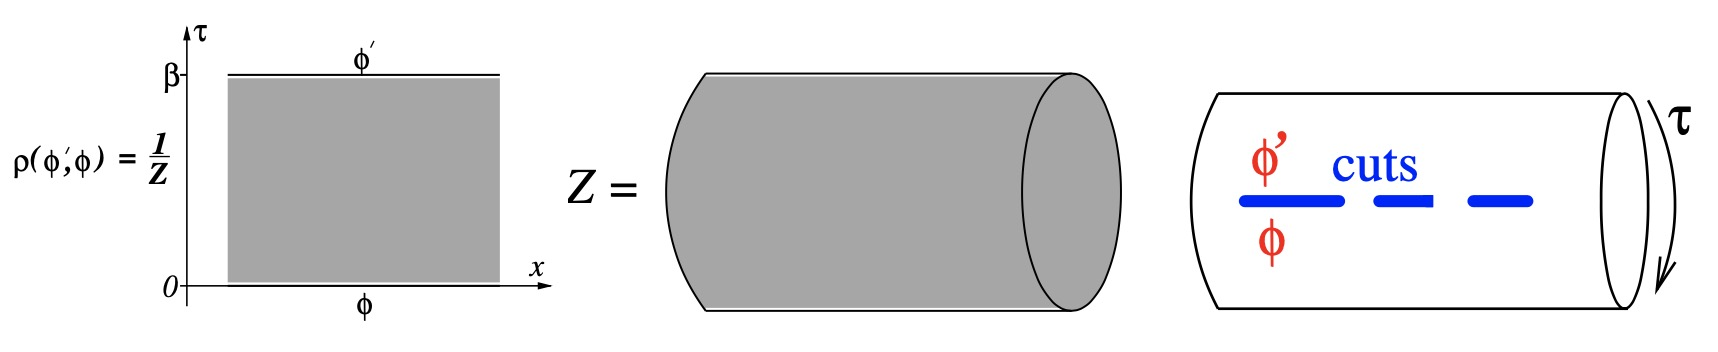
\includegraphics[width=0.9\linewidth]{pics/manifold.jpg}
\end{equation*}
We see that the reduced density matrix $\rho_A$ is obtained by sewing together only those points x which are not in $A$.
If we consider the ground state, just take $\beta$ to infinity and the manifold becomes the infinite plane.



\subsection{Replica Trick}
A closely related quantity for entanglement entropy is the Renyi entropy
\begin{equation}
	S_A^{(n)} = \frac{1}{1-n} \ln \Tr \rho_A^n.
\end{equation}
If the Renyi entropy is a analytic function of $n$, then the (von Neumann) entropy can be obtain by 
\begin{equation}
	S_A = \lim_{n\rightarrow 1}S_A^{(n)}.
\end{equation}
To proceed, we first consider the case where $n$ is integer, and then take the analytic continuation.
This correspond to the ``replica" system where we make $n$ copies of the fields, with proper boundary condition.
For the single-interval case, the boundary condition can be graphically represented as an $n$-sheeted Riemann surface:
\begin{equation*}
	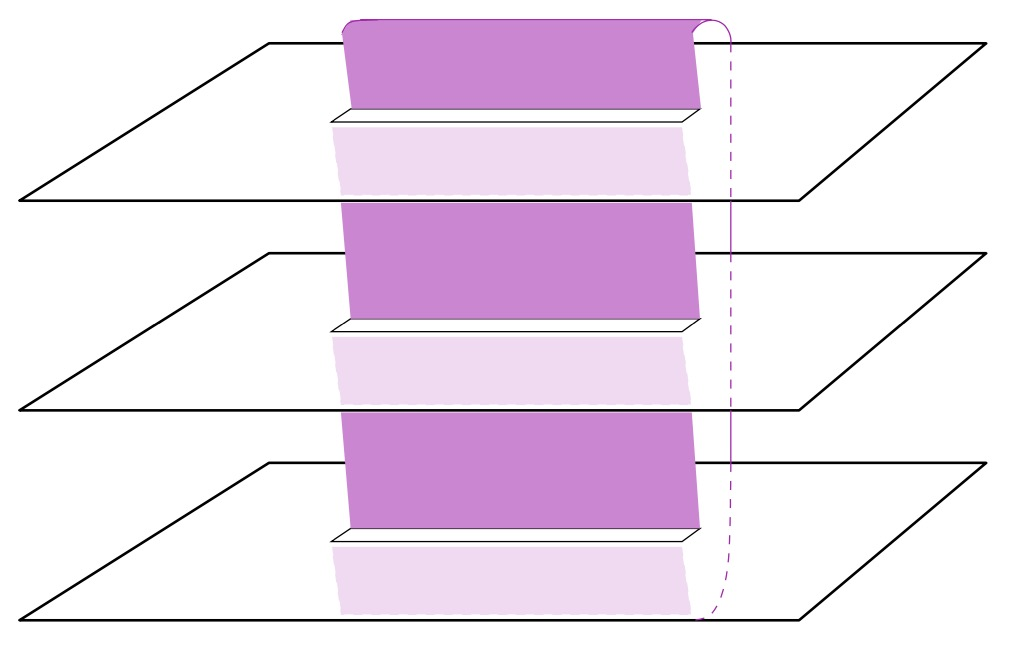
\includegraphics[width=0.3\linewidth]{pics/Riemannsurf.jpg}
\end{equation*}
Each layer correspond to different copy of field.
The bulk theory of the the system is just $n$ copy of the original Lagrangian, while the boundary condition introduced a brach cut to the theory.

\subsection{Twisted Fields}
Cardy et al. proposed that the field theory can be well described by inserting the \textit{twist fields} $\mathcal T_n$, $\tilde{\mathcal T}_n$ to each of the n disconnected sheets.
The partition function and other expectation values (on a single sheet) can be expressed as:
\begin{equation}
	Z_n = \langle \mathcal{T}_n(u) \tilde{\mathcal{T}}_n(v)\rangle, \quad
	\langle O(x,\tau)\rangle = \frac{1}{Z_n}\langle\mathcal{T}_n(u) \tilde{\mathcal{T}}_n(v) O(x,\tau) \rangle.
\end{equation}
One of the most important operator in the conformal field theory is the energy momentum tensor $T(z)$.
The expectation value for energy momentum tensor can be obtain by consider the conformal mapping
\begin{equation}
	z \rightarrow w(z) = \left(\frac{z-u}{z-v}\right)^{\frac{1}{n}}.
\end{equation} 
One can check that $w$ maps the Riemann surface to a single complex plane.
The energy-momentum tensors on different manifold are related by
\begin{equation}
	\langle T(z) \rangle = \left(\frac{d w}{d z}\right)^{2} \langle T(w)\rangle + \frac{c}{12}\{w, z\},
\end{equation}
where the Schwarzian derivative $\{z, w\}$ is
\begin{equation}
\begin{aligned}
	\{w,z\} &= \left(\frac{dw}{dz}\right)^{-2} \left[\frac{d^3 w}{dz^3}\frac{dw}{dz} - \frac{3}{2}\left(\frac{d^2 w}{dz^2}\right)^2\right] \\
	&= \frac{1}{2}\left(1-\frac{1}{n^2}\right)\frac{(u-v)^2}{(z-u)^2(z-v)^2}.
\end{aligned}
\end{equation}
The energy-momentum tensor on the complex plane is zero: $\langle T(w)\rangle=0$, so that on the Riemann surface is
\begin{equation}
	\frac{\langle\mathcal{T}_n(u) \tilde{\mathcal{T}}_n(v) T(z) \rangle}{\langle\mathcal{T}_n(u) \tilde{\mathcal{T}}_n(v) \rangle} 
	= \frac{c}{24}\left(1-\frac{1}{n^2}\right)\frac{(u-v)^2}{(z-u)^2(z-v)^2}.
\end{equation}
If we assume the twist field is primary, with dimension $d_n$, the two point function is\footnote{We focus on the holomorphic part, and assume the anti-holomorphic part has the same dimensionality. Also note that we have chosen a proper normalization for the twist fields.}
\begin{equation}
	\langle\mathcal{T}_n(u) \tilde{\mathcal{T}}_n(v) \rangle
	= (u-v)^{-2d_n}.
\end{equation}
And we also have the conformal Ward identity
\begin{equation}
\begin{aligned}
	\langle\mathcal{T}_n(u) \tilde{\mathcal{T}}_n(v) T(z) \rangle
	&= \left[\frac{\partial_u}{z-u} +\frac{d_n}{(z-u)^{2}}+\frac{\partial_v}{z-v} + \frac{d_n}{(z-v)^{2}}\right] \left\langle\mathcal{T}_{n}(u) \tilde{\mathcal{T}}_{n}(v)\right\rangle \\
	&= d|u-v|^{2-2d}
\end{aligned}
\end{equation}
Together we know
\begin{equation}
	d_n = \frac{c}{24}\left(1-\frac{1}{n^2}\right).
\end{equation}

\section{Entanglement Entropy}

\subsection{Single interval on an infinite chain}
Now note that the partition function for the replica system is related to the Renyi entropy by:
\begin{equation}
	\frac{Z_n}{Z^n} \propto \Tr \rho_A^n = c_n \left|\frac{u-v}{a}\right|^{-4n d_n},
\end{equation}
where $a$ is the UV cutoff introduced by $Z^n$.
The $n$-th order Renyi entropy is then
\begin{equation}
	S^{(n)}_A = \frac{c}{6}\left(1+\frac{1}{n}\right) \ln \left|\frac{u-v}{a}\right| + \frac{\ln c_n}{1-n}.
\end{equation}
As discussed, the entanglement entropy is obtained by taking the limit
\begin{equation}
	\lim_{n\rightarrow 1} S^{(n)}_A = \frac{c}{3}\ln\left|\frac{u-v}{a}\right| - c'_1.
\end{equation}
We thus obtained the entanglement entropy behavior of the single interval with length $l$:
\begin{equation}
	S_A = \frac{c}{3}\ln\frac{l}{a} + O(1).
\end{equation}


\subsection{Finite size and finite temperature}

We can also obtain the exact form of entanglement entropies for finite size or finite temperature, using a special conformal mapping that map the complex plane to a infinite cylinder with circumference $\beta$:
\begin{equation*}
	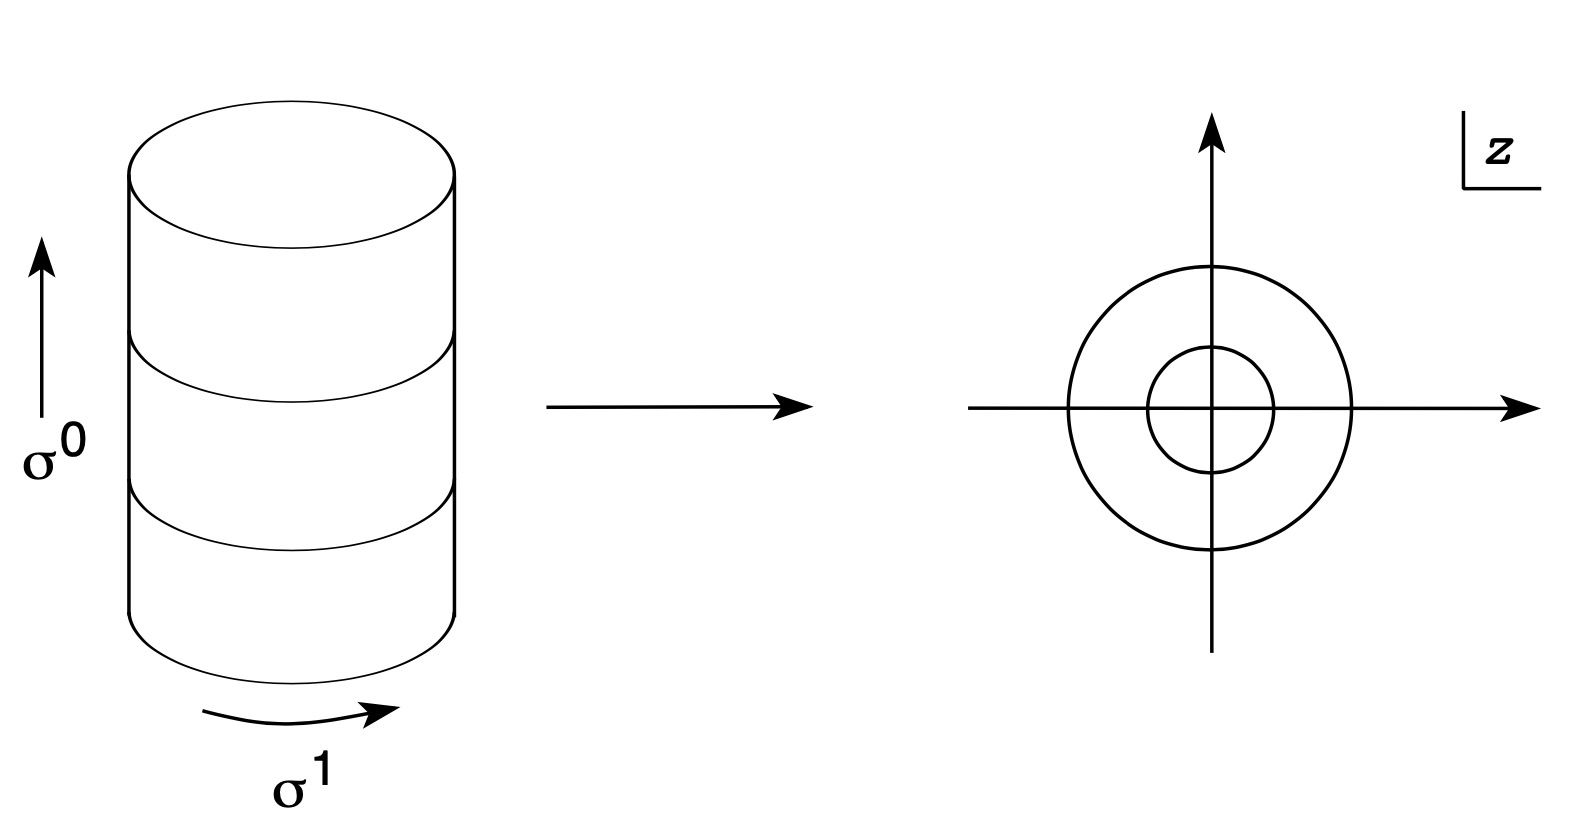
\includegraphics[width=0.45\linewidth]{pics/cyldrmap.jpg}
\end{equation*}
Specifically, $w$ and $z$ are related by:
\begin{equation}
	w = \frac{\beta}{2\pi} \ln z, \quad
	z = \exp\left(\frac{2\pi w}{\beta}\right).
\end{equation}
There are different ways to place $u$ and $v$.
If we place them along the radius, their image then lie parallel to the axis of the cylinder (the images are denoted as $w_1$ and $w_2$ respectively).
This correspond to the infinite chain with finite temperature.
The two point function is
\begin{equation}
\begin{aligned}
	\langle \mathcal{T}_n(w_1) \tilde{\mathcal T_n}(w_2)\rangle
	&= \left[w'(z_1)w'(z_2)\right]^{-d_n} \langle \mathcal{T}_n(z_1) \tilde{\mathcal T_n}(z_2)\rangle \\
	&= \exp \left[\frac{2\pi}{\beta} d_n(w_1+w_2)\right] \left[\exp\left(\frac{2\pi}{\beta} w_1\right)-\exp\left(\frac{2\pi}{\beta} w_2\right)\right]^{-2d_n} \\
	&= \left\{2\sinh\left[\frac{\pi(w_1-w_2)}{\beta}\right]\right\}^{-2d_n}.
\end{aligned}
\end{equation}
Similarly we have
\begin{equation}
	\Tr \rho_A^n = c_n \left[\frac{2}{b(\beta)}\sinh\left(\frac{\pi l}{\beta}\right)\right]^{-4nd_n}.
\end{equation}
The $b(\beta)$ is a $\beta$-dependent cutoff that should have the asymptotic behavior
\begin{equation}
	\lim_{\beta \rightarrow \infty} \frac{2}{b(\beta)}\sinh\left(\frac{\pi l}{\beta}\right) = \frac{l}{a} 
	\quad \Longrightarrow \quad
	b(\beta) = \frac{2\pi a}{\beta}.
\end{equation}
Thus the Renyi entropy for the replica system is
\begin{equation}
	S_A^{(n)} = \frac{c}{6}\left(1+\frac{1}{n}\right) \ln \left[\frac{\beta}{\pi a}\sinh\left(\frac{\pi l}{\beta}\right)\right] + \frac{\ln c_n}{1-n}.
\end{equation}
The entanglement entropy from the replica limit is
\begin{equation}
	S_A = \frac{c}{3} \ln \left[\frac{\beta}{\pi a}\sinh\left(\frac{\pi l}{\beta}\right)\right] + O(1).
\end{equation}

Apart from this, we can also place $u$ and $v$ on the same circle so that their image is perpendicular to the axis of the cylinder.
The calculation carries out without a change, but now $\beta$ is regarded as the system size (periodic boundary condition) while the temperature is zero.
We usually denote the size of the finite chain as $L$, so the finite-size result is:
\begin{equation}
	S_A = \frac{c}{3} \ln \left[\frac{L}{\pi a}\sinh\left(\frac{\pi l}{L}\right)\right] + O(1).
\end{equation}



\section{Quench Dynamics}








\end{document}


